\chapter{Blended Wing-Body cabin design review}
\markboth{Blended Wing-Body cabin design review}{Blended Wing-Body cabin design review}
\label{app:bwb_cabin_design}

The three configurations are presented and schematically described below. 

\section{Integrated structure}
\label{sec:app1_integrated_struct}

This concept consists on a unique skin which carries out the aerodynamics and the pressurization loads. 
The aerodynamisc envelop is divided by several walls to increase the stiffness.
The skin is optimized with respect to aero loads, which entails the skin is not optimized for the pressure. 
Indeed, this configuration is very simple and mimics conventional fuselages, both for the integrating vessel and the passengers' evacuation. 
The main issue is in the pressure load distribution: the pressure cabin is interrupted by structural elements which impacts negatively the passengers comfort. 
However, educing them to improve the comfort reduces the structural efficiency too, so a compromise has to be found.
\begin{figure}[h!]
	\centering
	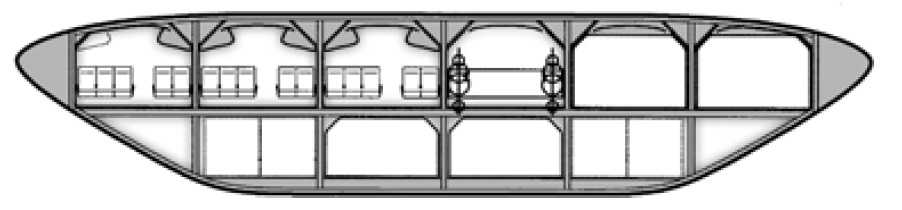
\includegraphics[keepaspectratio, width=0.6\textwidth]{images/app_bwb_cab/integrated_structure.jpg}
	\caption{Integrated cabin structure design.}
	\label{fig:bwb_integrated}
\end{figure}

\section{Segregated structure}
\label{sec:app1_segregated_struct}

This concept consists on a separation of the pressurization loads from all others. 
The structure is formed with two skins: the external skin which carries out the aerodynamics and the load transferring; and the internal one which only carries out the pressure load. Thus, the external skin is optimized with respect to aerodynamics and the internal one is formed by intersecting circular tubes which are connected with vertical shells. 
This solution is very efficient both aerodynamically and structurally, and it increases passengers comfort, but the double shell adds complexity in the overall design, with consequently penalties in weight. 
Also, the evacuation can be an issue, since the exit has to penetrate both the shells, a stiffener may be needed. 
\begin{figure}[h!]
	\centering
	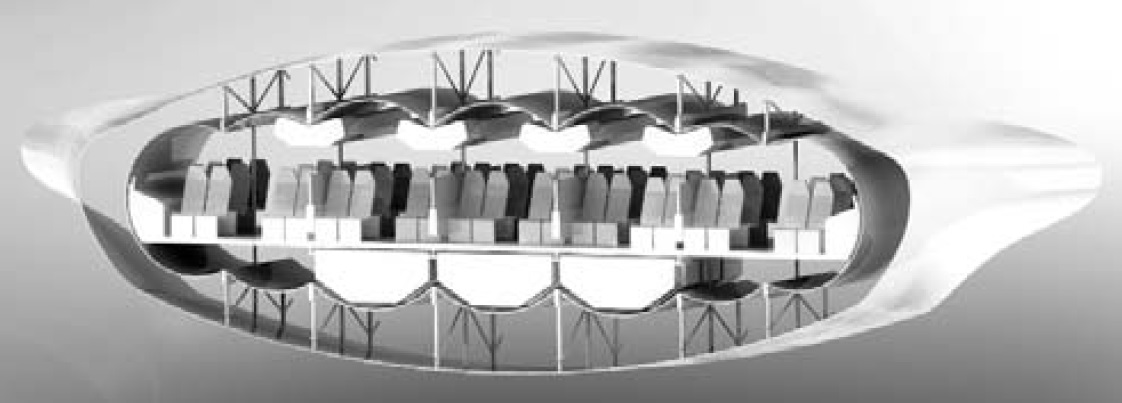
\includegraphics[keepaspectratio, width=0.6\textwidth]{images/app_bwb_cab/segregated_structure.jpg}
	\caption{Segregated cabin structure design.}
	\label{fig:bwb_segregated}
\end{figure}

\section{Oval structure}
\label{sec:app1_oval_struct}

Compared to the previous two, this configuration is the more complex: in every design phase a compromise between structural, aerodynamic efficiency and payload integration has to be found. It has shown the largest amount of pressurized space, introducing penalties in weight and in the aerodynamics design, which is compromised by structural requirements. 
The major interest of this configuration lies in the passengers comfort: they have an uninterrupted view in the pressure cabin which enhances their orientation and acceptance; it also allows natural light throughout the cabin. On this side, the oval configuration is the closest possible to a conventional fuselage. 
The evacuation is done in the same way as in the integrating concept, with cutaways in the outer shell. 
\begin{figure}[h!]
	\centering
	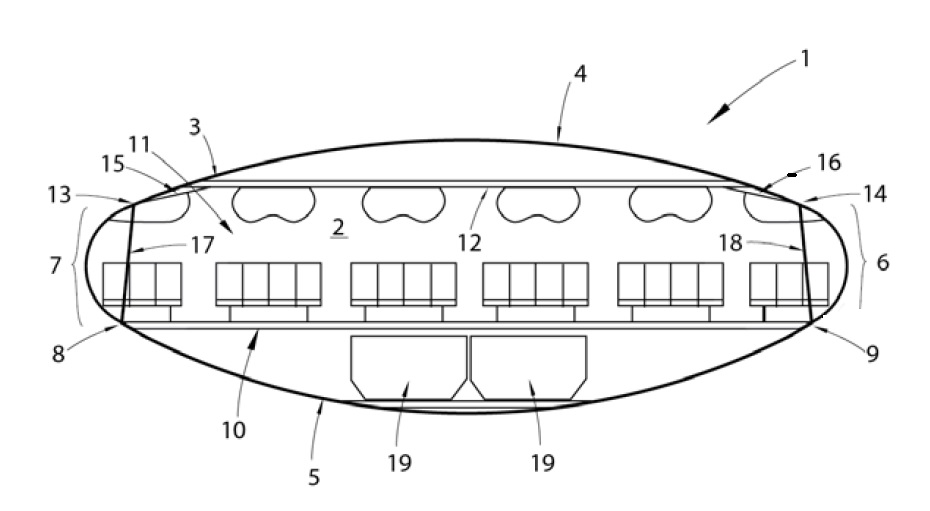
\includegraphics[keepaspectratio, width=0.6\textwidth]{images/app_bwb_cab/oval_structure.jpg}
	\caption{Oval cabin structure design.}
	\label{fig:bwb_oval}
\end{figure}
